\documentclass[12pt,letterpaper]{article}
\usepackage{graphicx,textcomp}
\usepackage{natbib}
\usepackage{setspace}
\usepackage[a4paper,margin=1in]{geometry}
\usepackage{color}
\usepackage[reqno]{amsmath}
\usepackage{amsthm}
\usepackage{fancyvrb}
\usepackage{amssymb,enumerate}
\usepackage[all]{xy}
\usepackage{endnotes}
\usepackage{lscape}
\newtheorem{com}{Comment}
\usepackage{float}
\usepackage{hyperref}
\newtheorem{lem} {Lemma}
\newtheorem{prop}{Proposition}
\newtheorem{thm}{Theorem}
\newtheorem{defn}{Definition}
\newtheorem{cor}{Corollary}
\newtheorem{obs}{Observation}
\usepackage[compact]{titlesec}
\usepackage{dcolumn}
\usepackage{tikz}
\usetikzlibrary{arrows}
\usepackage{multirow}
\usepackage{xcolor}
\newcolumntype{.}{D{.}{.}{-1}}
\newcolumntype{d}[1]{D{.}{.}{#1}}
\definecolor{light-gray}{gray}{0.65}
\usepackage{url}
\usepackage{listings}
\usepackage{color}

\definecolor{codegreen}{rgb}{0,0.6,0}
\definecolor{codegray}{rgb}{0.5,0.5,0.5}
\definecolor{codepurple}{rgb}{0.58,0,0.82}
\definecolor{backcolour}{rgb}{0.95,0.95,0.92}

\lstdefinestyle{mystyle}{
	backgroundcolor=\color{backcolour},   
	commentstyle=\color{codegreen},
	keywordstyle=\color{magenta},
	numberstyle=\tiny\color{codegray},
	stringstyle=\color{codepurple},
	basicstyle=\footnotesize,
	breakatwhitespace=false,         
	breaklines=true,                 
	captionpos=b,                    
	keepspaces=true,                 
	numbers=left,                    
	numbersep=5pt,                  
	showspaces=false,                
	showstringspaces=false,
	showtabs=false,                  
	tabsize=2
}
\lstset{style=mystyle}
\newcommand{\Sref}[1]{Section~\ref{#1}}
\newtheorem{hyp}{Hypothesis}

\title{Problem Set 1}
\date{Due: October 9, 2025}
\author{Applied Stats/Quant Methods 1}

\begin{document}
	\maketitle
	
	\section*{Instructions}
	\begin{itemize}
	\item Please show your work! You may lose points by simply writing in the answer. If the problem requires you to execute commands in \texttt{R}, please include the code you used to get your answers. Please also include the \texttt{.R} file that contains your code. If you are not sure if work needs to be shown for a particular problem, please ask.
\item Your homework should be submitted electronically on GitHub.
\item This problem set is due before 23:59 on Thursday October 9, 2025. No late assignments will be accepted.
	\end{itemize}
	
	\vspace{1cm}
	\section*{Question 1: Education}

A school counselor was curious about the average of IQ of the students in her school and took a random sample of 25 students' IQ scores. The following is the data set:\\
\vspace{.5cm}

\lstinputlisting[language=R, firstline=36, lastline=36]{PS01_DP.R}  

\vspace{1cm}

\begin{enumerate}
	\item Find a 90\% confidence interval for the average student IQ in the school.\\
	
	\item Next, the school counselor was curious  whether  the average student IQ in her school is higher than the average IQ score (100) among all the schools in the country.\\ 
	
	\noindent Using the same sample, conduct the appropriate hypothesis test with $\alpha=0.05$.
\end{enumerate}

\newpage
	\section*{Solution - Question 1: Education}
\vspace{.5cm}
\subsection*{1. Confidence Interval}
\begin{itemize}
	\item 
	Calculate the mean 
	\lstinputlisting[language=R, firstline=39, lastline=40]{PS01_DP.R} 
  \begin{verbatim}
  	[1] 98.44
  \end{verbatim}
  \item 
  Calculate the sum of the squared errors to get the variance, and then the standard deviation
  	\lstinputlisting[language=R, firstline=43, lastline=47]{PS01_DP.R} 
  \begin{verbatim}
  	[1] 13.09287
  \end{verbatim}
  \item 
  Calculate the standard error 
  \lstinputlisting[language=R, firstline=50, lastline=51]{PS01_DP.R} 
  \begin{verbatim}
  	[1] 2.618575
  \end{verbatim}
   \item 
  Find the t-score for the desired confidence level, with 24 degrees of freedom
  \lstinputlisting[language=R, firstline=54, lastline=55]{PS01_DP.R} 
  \begin{verbatim}
  	[1] 1.710882
  \end{verbatim}
   \item 
  Construct the confidence interval by calculating its lower and upper limits
  \lstinputlisting[language=R, firstline=58, lastline=61]{PS01_DP.R} 
  \begin{verbatim}
  	> lowerlimit
  	[1] 93.95993
  	> upperlimit
  	[1] 102.9201
  \end{verbatim}
  \end{itemize}
\newpage 
\subsection*{2. Hypothesis Testing}\\
\begin{itemize}
	\item \textbf{Step 1:} assumptions\\
	\begin{itemize}
		\item the data is quantitative
		\item the sampling method is random
		\item the sample size is smaller than 30, so we cannot assume it follows a normal distribution - therefore, I used the t-score and not the Z-score as the test statistic 
	\end{itemize}
	\item \textbf{Step 2:} hypotheses\\
	\begin{itemize}
		\item \textbf{Null hypothesis:} the mean is lower or equal to 100 
		\item \textbf{Alternative hypothesis:} the mean is higher than 100 
	\end{itemize}
	\item \textbf{Step 3: } calculate the test statistic\\
		\lstinputlisting[language=R, firstline=70, lastline=71]{PS01_DP.R} 
		\begin{verbatim}
			[1] -0.5957439
		\end{verbatim}
	\item \textbf{Step 4:} calculate the p-value \\
	\lstinputlisting[language=R, firstline=74, lastline=75]{PS01_DP.R} 
	\begin{verbatim}
		[1] 0.7215383
	\end{verbatim}
	\item \textbf{Step 5:} draw a conclusion \\
	The p-value is higher than alpha, so we cannot reject the null hypothesis that the mean is lower or equal to 100 
\end{itemize}

\newpage
	\section*{Question 2: Political Economy}

\noindent Researchers are curious about what affects the amount of money communities spend on addressing homelessness. The following variables constitute our data set about social welfare expenditures in the USA. \\
\vspace{.5cm}


\begin{tabular}{r|l}
	\texttt{State} &\emph{50 states in US} \\
	\texttt{Y} & \emph{per capita expenditure on shelters/housing assistance in state}\\
	\texttt{X1} &\emph{per capita personal income in state} \\
	\texttt{X2} &  \emph{Number of residents per 100,000 that are "financially insecure" in state}\\
	\texttt{X3} &  \emph{Number of people per thousand residing in urban areas in state} \\
	\texttt{Region} &  \emph{1=Northeast, 2= North Central, 3= South, 4=West} \\
\end{tabular}

\vspace{.5cm}
\noindent Explore the \texttt{expenditure} data set and import data into \texttt{R}.
\vspace{.5cm}
\lstinputlisting[language=R, firstline=54, lastline=54]{PS01_DP.R}  
\vspace{.5cm}
\begin{itemize}

\item
Please plot the relationships among \emph{Y}, \emph{X1}, \emph{X2}, and \emph{X3}? What are the correlations among them (you just need to describe the graph and the relationships among them)?
\vspace{.5cm}
\item
Please plot the relationship between \emph{Y} and \emph{Region}? On average, which region has the highest per capita expenditure on housing assistance?
\vspace{.5cm}
\item
Please plot the relationship between \emph{Y} and \emph{X1}? Describe this graph and the relationship. Reproduce the above graph including one more variable \emph{Region} and display different regions with different types of symbols and colors.
\end{itemize}
\newpage
	\section*{Solution - Question 2: Political Economy}
\begin{figure}[h!]\centering
	\caption{\footnotesize Scatterplot of X1 and Y}
	\label{fig:plot_1}
	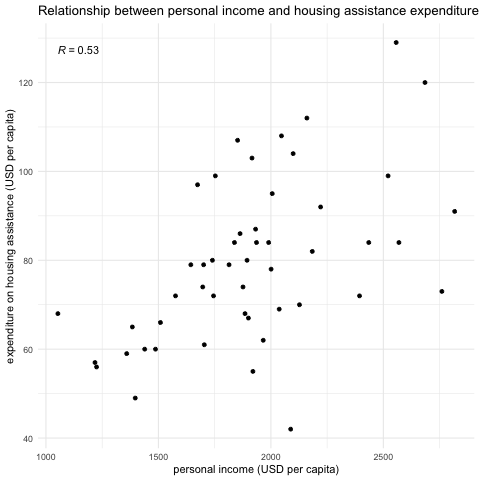
\includegraphics[width=.95\textwidth]{scatter_x1_y.png}
\end{figure} 
\textbf{Interpretation:} \\ There is a moderate positive association between the personal income and the expenditure on housing assistance in a state, both measured in USD per capita. The Pearson correlation coefficient points towards the same conclusion, as its value is above 0, but not close enough to 1 to suggest a strong association between the two variables. 
\newpage
\begin{figure}[h!]\centering
	\caption{\footnotesize Scatterplot of X2 and Y}
	\label{fig:plot_2}
	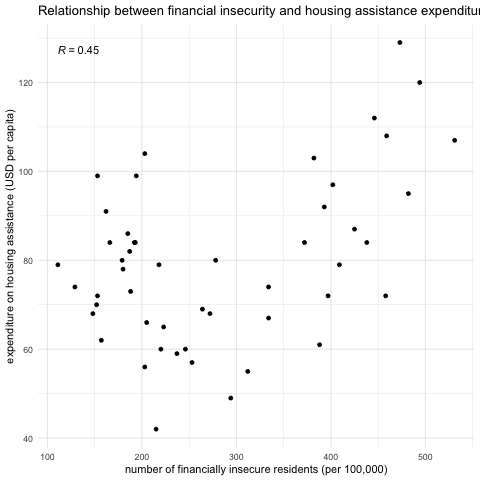
\includegraphics[width=.95\textwidth]{scatter_x2_y.png}
\end{figure}
\textbf{Interpretation:} There is a moderate positive association between the personal income and the expenditure on housing assistance in a state, both measured in USD per capita. The Pearson correlation coefficient points towards the same conclusion, as its value is above 0, but not close enough to 1 to suggest a strong association between the two variables. 
\newpage
\begin{figure}[h!]\centering
	\caption{\footnotesize Scatterplot of X3 and Y}
	\label{fig:plot_3}
	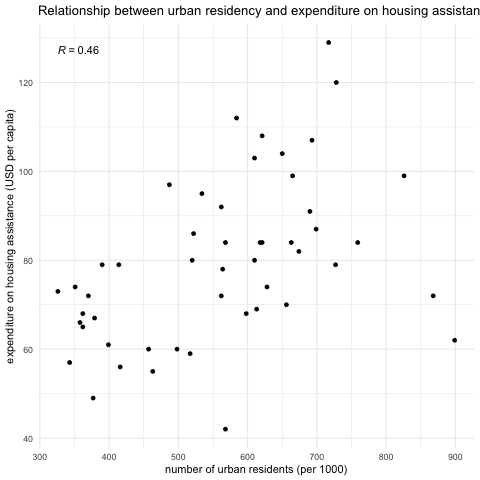
\includegraphics[width=.95\textwidth]{scatter_x3_y.png}
\end{figure}
\textbf{Interpretation:} There is a moderate positive association between the personal income and the expenditure on housing assistance in a state, both measured in USD per capita. The Pearson correlation coefficient points towards the same conclusion, as its value is above 0, but not close enough to 1 to suggest a strong association between the two variables. 
\newpage
\begin{figure}[h!]\centering
	\caption{\footnotesize Scatterplot of X1 and X2}
	\label{fig:plot_4}
	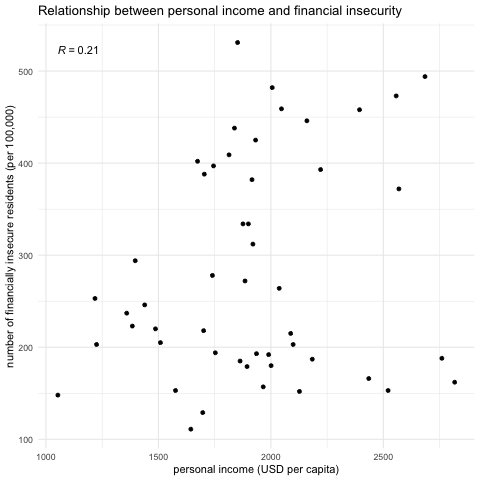
\includegraphics[width=.95\textwidth]{scatter_x1_x2.png}
\end{figure}
\textbf{Interpretation:} There is a moderate positive association between the personal income and the expenditure on housing assistance in a state, both measured in USD per capita. The Pearson correlation coefficient points towards the same conclusion, as its value is above 0, but not close enough to 1 to suggest a strong association between the two variables. 
\newpage
\begin{figure}[h!]\centering
	\caption{\footnotesize Scatterplot of X2 and X3}
	\label{fig:plot_5}
	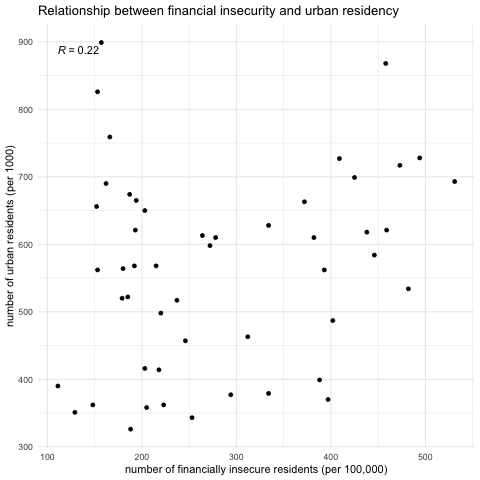
\includegraphics[width=.95\textwidth]{scatter_x2_x3.png}
\end{figure}
\textbf{Interpretation:} There is a moderate positive association between the personal income and the expenditure on housing assistance in a state, both measured in USD per capita. The Pearson correlation coefficient points towards the same conclusion, as its value is above 0, but not close enough to 1 to suggest a strong association between the two variables. 
\newpage
\begin{figure}[h!]\centering
	\caption{\footnotesize Scatterplot of X2 and X3}
	\label{fig:plot_6}
	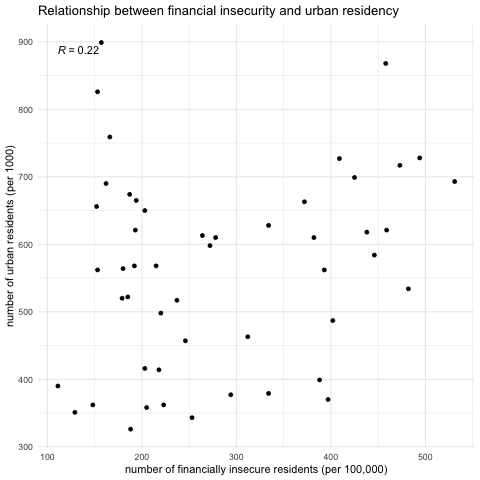
\includegraphics[width=.95\textwidth]{scatter_x2_x3.png}
\end{figure}
\textbf{Interpretation:} There is a moderate positive association between the personal income and the expenditure on housing assistance in a state, both measured in USD per capita. The Pearson correlation coefficient points towards the same conclusion, as its value is above 0, but not close enough to 1 to suggest a strong association between the two variables. 
\newpage
\begin{figure}[h!]\centering
	\caption{\footnotesize Scatterplot of X1 and X2}
	\label{fig:plot_7}
	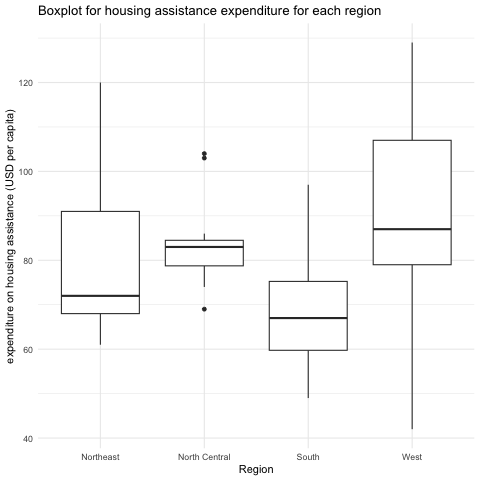
\includegraphics[width=.95\textwidth]{boxplot_reg_y.png}
\end{figure}
\textbf{Interpretation:} There is a moderate positive association between the personal income and the expenditure on housing assistance in a state, both measured in USD per capita. The Pearson correlation coefficient points towards the same conclusion, as its value is above 0, but not close enough to 1 to suggest a strong association between the two variables. 
\end{document}

